\chapter{动机}\label{chap:motivation}

尽管内核分割技术能带来显著的性能提升,实现这项技术的困难阻碍了开发人员广泛使用这一技术。

\begin{figure}[htbp]
    \centering
    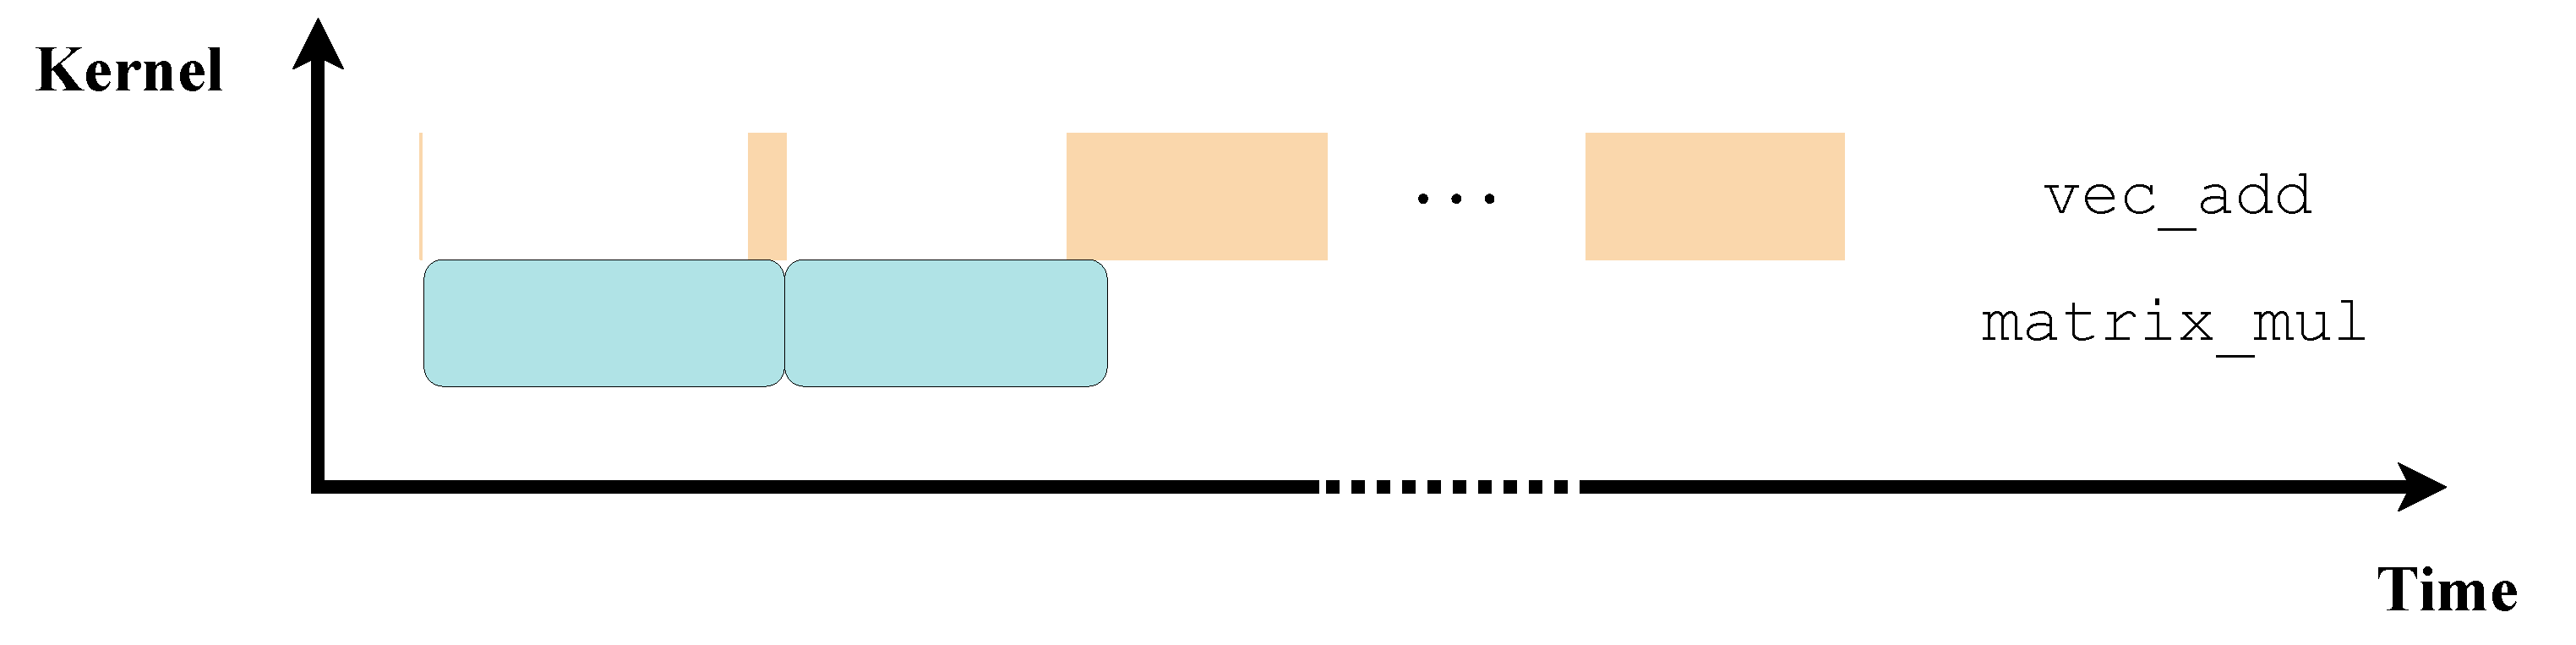
\includegraphics[width=0.9\linewidth]{bad_cosched/bad_cosched.drawio.pdf}
    \caption{内核分割后并行执行的时间线。在这种分割下未实现性能提升。\texttt{vec\_add}的部分执行过程在图中未展示。}
    \label{bad-cosched}    
\end{figure}

首先,开发人员需要将完整kernel改写为若干subkernel,增加了代码复杂性。许多设备代码的运行依赖于\texttt{threadIdx}, \texttt{blockIdx},因此实现子内核时也需要将这些索引转换为原kernel中的索引。如\autoref{code:naivedevicecudacode}的每个block负责处理输入矩阵的不同子矩阵,每个thread通过\texttt{thread/blockIdx}确定自身需要处理的数据范围。若将kernel分割,仅凭\texttt{thread/blockIdx}无法获知thread处理的数据范围,因为属于不同的subkernel的thread可能具有相同的\texttt{thread/blockIdx}。其次,选择合适的子内核大小(以下称为\emph{分割参数})并非易事。若子内核包含block数目过多,设备将缺少用于执行其他子内核的资源,进而无法与其他kernel并行;若子内核包含block数目过少,则kernel会被划分为众多subkernel,而过多的subkernel启动开销会抵消并行带来的性能提升。如\autoref{bad-cosched}所示,错误的分割方式使得kernel并未实现并行,反而引入了多次内核启动的开销,使得性能低于未分割内核的情况。此外,GPU架构对subkernel大小的选择有巨大影响。由于不同类型的GPU含有的硬件资源不同,并行的不同kernel线程数目最佳比例也会受到影响。在不同硬件运行时,同一程序可能表现出不同的特性\cite{10.1145/1498765.1498785}\cite{KONSTANTINIDIS201737}。例如,程序在某GPU架构下为内存密集型应用,而在另一架构下表现为计算密集型应用。这要求开发人员在开发通用的程序时对不同设备进行多次性能分析以获得合适的分割参数,增加了开发时的负担。

\begin{figure}[htbp]
    \centering
    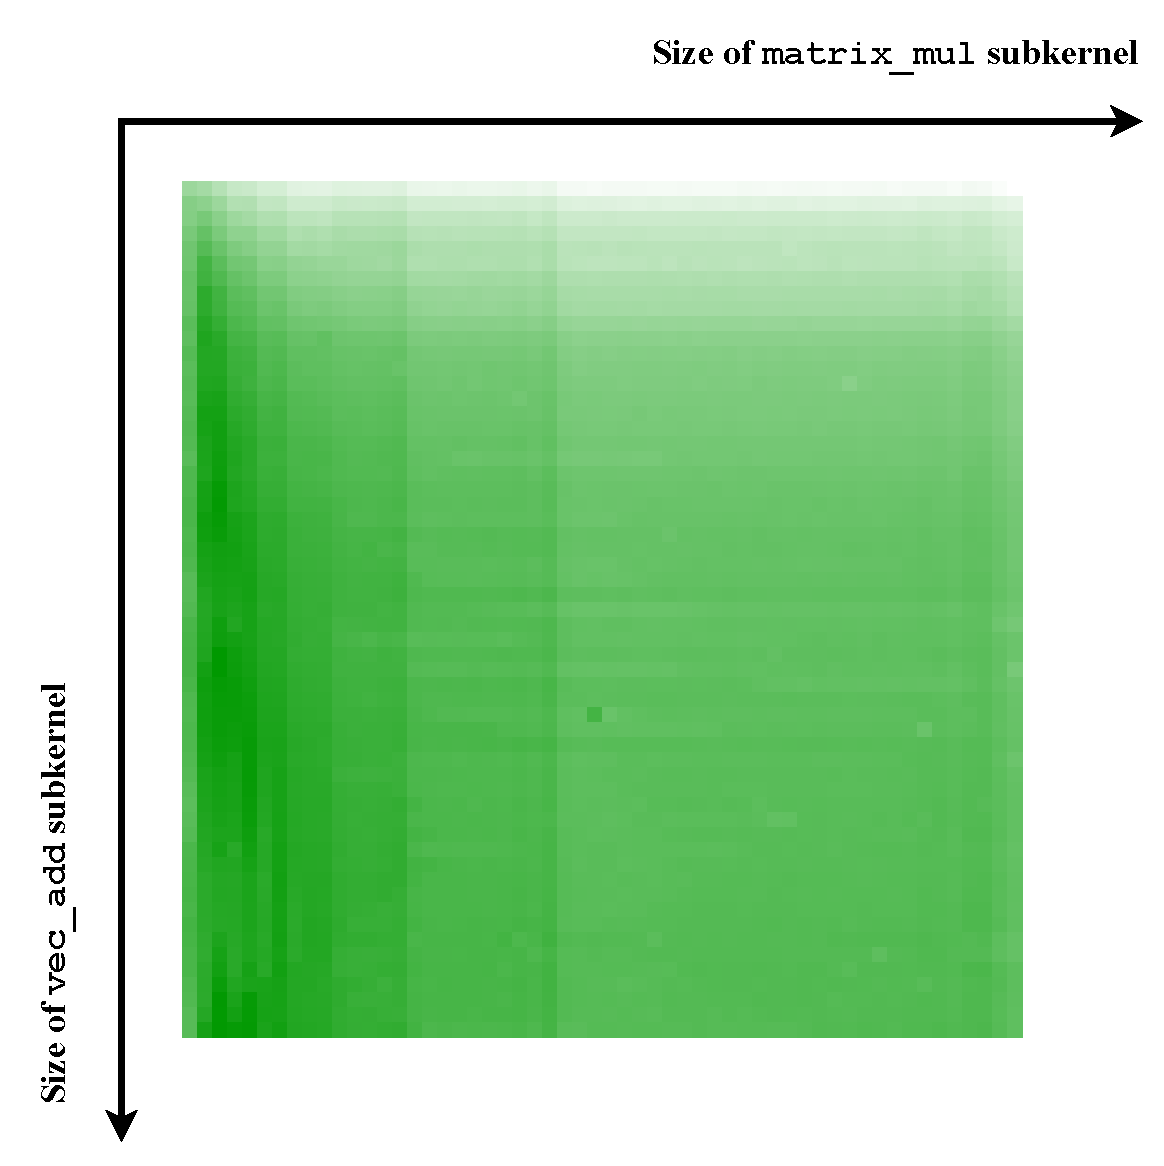
\includegraphics[width=0.8\linewidth]{consistency/consistency.drawio.pdf}
    \caption{不同分割参数下的性能。纵轴表示\texttt{vec\_add}的子内核大小(即所含block数目),横轴表示\texttt{matrix\_mul}的子内核大小,每个坐标对应的方格颜色表示在此分割参数的组合下的程序性能,颜色越深表示性能越高。}
    \label{consistency}
\end{figure}

由于可选的分割参数组合众多,选择合适的分割参数是具有挑战的。但分割参数与在该参数下的性能间存在特定规律。为简化分析,本文只考虑2个kernel并行的情形,对多kernel并行的研究将作为后续工作。我们测试了\texttt{vec\_add}和\texttt{matrix\_mul}在不同分割下并行的性能,\autoref{consistency}展示了此实验的结果。图中纵轴表示\texttt{vec\_add}的子内核大小(即所含block数目),横轴表示\texttt{matrix\_mul}的子内核大小,每个坐标对应的方格颜色表示在此分割参数的组合下的程序性能,颜色越深表示性能越高。图中信息表明,当分割参数变化时,程序性能的变化具有连续性。即,当分割参数发生微小变化时,程序性能也会相应发生微小变动,而不会出现剧烈的波动。这种连续性允许我们类比数值计算中求解函数极值的算法(如梯度下降)来寻找性能较高的配置,而无需遍历地测试每一种可能的分割方式,大大降低了开发负担。本文提出的ko-Sched即受此启发,以较低开销寻找高性能分割参数,同时保证性能与最佳分割方式相当。